\documentclass{beamer}
\usepackage[utf8]{inputenc}
\usetheme{Madrid}
\usecolortheme{default}
\usepackage{amsmath,amssymb,amsfonts,amsthm}
\usepackage{txfonts}
\usepackage{tkz-euclide}
\usepackage{listings}
\usepackage{adjustbox}
\usepackage{array}
\usepackage{tabularx}
\usepackage{gvv}
\usepackage{lmodern}
\usepackage{circuitikz}
\usepackage{tikz}
\usepackage{graphicx}
\usepackage[T1]{fontenc}

\setbeamertemplate{page number in head/foot}[totalframenumber]

\usepackage{tcolorbox}
\tcbuselibrary{minted,breakable,xparse,skins}



\definecolor{bg}{gray}{0.95}
\DeclareTCBListing{mintedbox}{O{}m!O{}}{%
  breakable=true,
  listing engine=minted,
  listing only,
  minted language=#2,
  minted style=default,
  minted options={%
    linenos,
    gobble=0,
    breaklines=true,
    breakafter=,,
    fontsize=\small,
    numbersep=8pt,
    #1},
  boxsep=0pt,
  left skip=0pt,
  right skip=0pt,
  left=25pt,
  right=0pt,
  top=3pt,
  bottom=3pt,
  arc=5pt,
  leftrule=0pt,
  rightrule=0pt,
  bottomrule=2pt,
  toprule=2pt,
  colback=bg,
  colframe=orange!70,
  enhanced,
  overlay={%
    \begin{tcbclipinterior}
    \fill[orange!20!white] (frame.south west) rectangle ([xshift=20pt]frame.north west);
    \end{tcbclipinterior}},
  #3,
}
\lstset{
    language=C,
    basicstyle=\ttfamily\small,
    keywordstyle=\color{blue},
    stringstyle=\color{orange},
    commentstyle=\color{green!60!black},
    numbers=left,
    numberstyle=\tiny\color{gray},
    breaklines=true,
    showstringspaces=false,
}


\title {2.6.39}
\date{August 31,2025}


\author 
{Manohar-AI25BTECH11028}



\begin{document}


\frame{\titlepage}
\begin{frame}{Question}
The area of the quadrilateral ABCD, where A(0,4,1), B(2,3,-1), C(4,5,0) and D(2,6,2), is equal to
\end{frame}





\begin{frame}{Equation}
The area of a quadrilateral is given by half the magnitude of the cross product of its diagonals.  

First, we find the vectors for the diagonals  
\begin{align*}
 \vec{P} &= \vec{C} - \vec{A} = \myvec{4\\5\\0} - \myvec{0\\4\\1} = \myvec{4\\1\\-1} \\
 \vec{Q} &= \vec{D} - \vec{B} = \myvec{2\\6\\2} - \myvec{2\\3\\-1} = \myvec{0\\3\\3} 
\end{align*}
\end{frame}
\begin{frame}{Solution}

Now, we compute the cross product $\vec{P} \times \vec{Q}$ using the determinant expansion:  

\begin{align*}
\vec{P} \times \vec{Q} &= 
\myvec{
\left|\myvec{1 & 3 \\ -1 & 3}\right| \\
-\left|\myvec{4 & 3 \\ -1 & 3}\right| \\
\left|\myvec{4 & 1 \\ 0 & 3}\right|
} \\
&= \myvec{(1)(3) - (3)(-1) \\ -( (4)(3) - (3)(-1)) \\ (4)(3) - (1)(0)} \\
&= \myvec{6 \\ -12 \\ 12}
\end{align*}
\end{frame}

\begin{frame}{Solution}
The area is half the magnitude of this vector:  

\begin{align*}
\text{Area} &= \tfrac{1}{2} \|\vec{P} \times \vec{Q}\| \\
&= \tfrac{1}{2} \sqrt{6^2 + (-12)^2 + 12^2} \\
&= \tfrac{1}{2} \sqrt{36 + 144 + 144} \\
&= \tfrac{1}{2} \sqrt{324} \\
&= \tfrac{1}{2}(18) \\
&= 9
\end{align*}

Thus, the area of the quadrilateral is 9 square units.

\end{frame}



\begin{frame}[fragile]
    \frametitle{C Code}

    \begin{lstlisting}

// quad_area.c
#include <math.h>

double quad_area(double Px, double Py, double Pz, double Qx, double Qy, double Qz) {
    // cross product components
    double cx = Py*Qz - Pz*Qy;
    double cy = Pz*Qx - Px*Qz;
    double cz = Px*Qy - Py*Qx;

    // magnitude of cross product
    double magnitude = sqrt(cx*cx + cy*cy + cz*cz);

    // area = half the magnitude
    return 0.5 * magnitude;
}


    

    \end{lstlisting}
\end{frame}



\begin{frame}[fragile]
    \frametitle{Python+C Code}
    \begin{lstlisting}
    
 import ctypes
import matplotlib.pyplot as plt
import numpy as np

# Load shared library
lib = ctypes.CDLL("./quad_area.so")   # use quad_area.dll on Windows

# Function signature
lib.quad_area.restype = ctypes.c_double
lib.quad_area.argtypes = [ctypes.c_double, ctypes.c_double, ctypes.c_double,
                          ctypes.c_double, ctypes.c_double, ctypes.c_double]





    \end{lstlisting}
\end{frame}

\begin{frame}[fragile]
    \frametitle{Python+C Code}
    \begin{lstlisting}

# Points A, B, C, D
A = np.array([0, 4, 1])
B = np.array([2, 3, -1])
C = np.array([4, 5, 0])
D = np.array([2, 6, 2])

# Diagonals
P = C - A
Q = D - B

# Call C function
area = lib.quad_area(P[0], P[1], P[2], Q[0], Q[1], Q[2])
print("Area (from C via ctypes) =", area)


    \end{lstlisting}
\end{frame}

\begin{frame}[fragile]
    \frametitle{Python+C Code}
    \begin{lstlisting}
# --- Plot quadrilateral ---
fig = plt.figure()
ax = fig.add_subplot(111, projection="3d")

# Connect vertices in order A-B-D-C-A
X = [A[0], B[0], C[0], D[0], A[0]]
Y = [A[1], B[1], C[1], D[1], A[1]]
Z = [A[2], B[2], C[2], D[2], A[2]]

ax.plot(X, Y, Z, 'b-', marker='o')
ax.set_xlabel("X-axis")
ax.set_ylabel("Y-axis")
ax.set_zlabel("Z-axis")
    \end{lstlisting}
\end{frame}


\begin{frame}[fragile]
    \frametitle{Python+C Code}
    \begin{lstlisting}


# Save before show
plt.savefig("/storage/emulated/0/matrix/Matgeo/2.6.39/figs/Figure_1.png", dpi=300, bbox_inches='tight')
plt.show()
    \end{lstlisting}
\end{frame}


\begin{frame}{Plot}
    \centering
    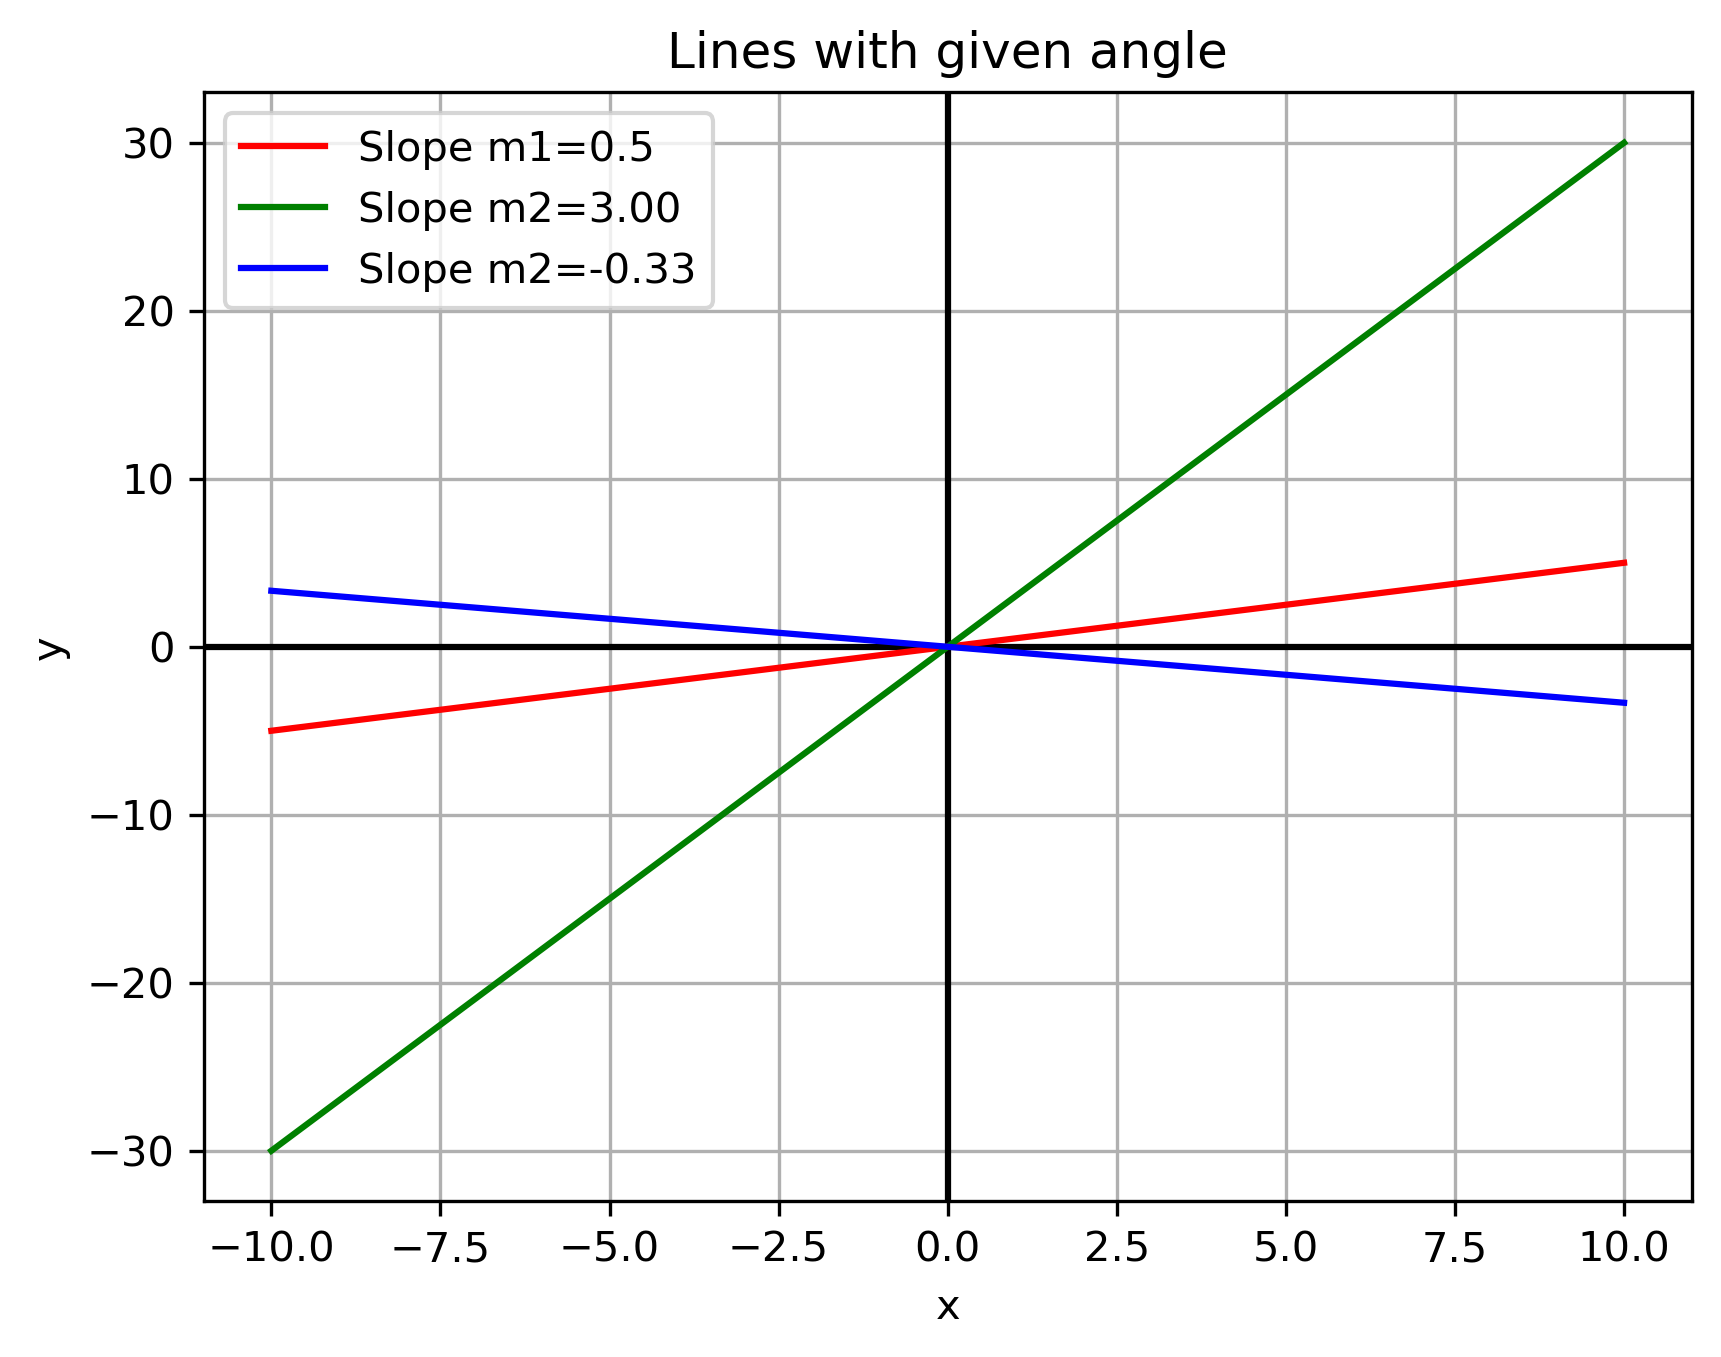
\includegraphics[width=\columnwidth, height=0.8\textheight, keepaspectratio]{figs/figure_1.png}     
\end{frame}

\begin{frame}[fragile]
    \frametitle{Python Code}
    \begin{lstlisting}
        import numpy as np
import matplotlib.pyplot as plt

# Points A, B, C, D
A = np.array([0, 4, 1])
B = np.array([2, 3, -1])
C = np.array([4, 5, 0])
D = np.array([2, 6, 2])

# Diagonals
P = C - A
Q = D - B

# Cross product & area
cross = np.cross(P, Q)
area = 0.5 * np.linalg.norm(cross)
print("Area (NumPy) =", area)


    \end{lstlisting}
\end{frame}

\begin{frame}[fragile]
    \frametitle{Python Code}
    \begin{lstlisting}
# --- Plot quadrilateral ---
fig = plt.figure()
ax = fig.add_subplot(111, projection="3d")

X = [A[0], B[0], C[0], D[0], A[0]]
Y = [A[1], B[1], C[1], D[1], A[1]]
Z = [A[2], B[2], C[2], D[2], A[2]]

ax.plot(X, Y, Z, 'r-', marker='o')
ax.set_xlabel("X-axis")
ax.set_ylabel("Y-axis")
ax.set_zlabel("Z-axis")

    \end{lstlisting}
\end{frame}

\begin{frame}[fragile]
    \frametitle{Python Code}
    \begin{lstlisting}
     # Save before show
plt.savefig("/storage/emulated/0/matrix/Matgeo/2.6.39/figs/Figure_1.png", dpi=300, bbox_inches='tight')
plt.show()   
    \end{lstlisting}
    
\end{frame}
\end{document}